\chapter{The Regression Line}

Do students who sleep more get better grades? Does a house with more square feet sell for more? In the
Scatter Plots and Correlation chapter, you measured how strongly two variables move together with the
correlation coefficient $r$. This chapter goes one step further: it finds the single straight line that best
fits the data, so you can use one variable to predict the other, and it shows how to judge whether that line
is any good.

\section{Linear Regression}

Suppose you wanted to predict a teacher's starting salary based on how many years
of experience they have. You might expect that more experience leads to a higher
salary, but how do you turn that intuition into a precise estimate? That is
exactly what a \newterm{linear regression model}\index{linear regression model}
does. It gives you a straight-line equation that describes the relationship between
two variables, so you can use the value of one to predict the value of the other.

\subsubsection{The Regression Model}

When one variable depends on or is explained by another, we call the variable being
predicted the \newterm{dependent variable}\index{dependent variable}. The variable doing the
explaining is the \newterm{independent variable}\index{independent variable}. In our example,
starting salary is the dependent (response) variable and years of experience is
the independent (explanatory) variable. It would make little sense to say that a teacher's salary determines
how many years they have worked.

The linear relation between two variables is described by the
\newterm{population regression equation}\index{population regression equation}:

\[
Y = \alpha + \beta X
\]

where $Y$ is the response variable, $X$ is the independent variable, $\alpha$ is
the \newterm{$y$-intercept}\index{y-intercept} (the value of $Y$ when $X = 0$),
and $\beta$ is the \newterm{slope}\index{slope} (the amount $Y$ changes for every
one-unit increase in $X$). This equation describes the true relationship in the
population, but in practice, we never know $\alpha$ and $\beta$ exactly. We
estimate them from sample data.

Once we have estimates for $\alpha$ and $\beta$, we can write the
\newterm{estimated regression line}\index{estimated regression line}:

\[
\hat{y} = a + bx
\]

The symbol $\hat{y}$ (read ``$y$-hat'') is the \newterm{predicted value}\index{predicted value}
of $Y$ for a given value of $X$. Notice the difference in notation: $\alpha$ and
$\beta$ are population parameters; $a$ and $b$ are their sample-based estimates.

Here is a quick reference for the symbols introduced so far in this chapter:

\begin{center}
\begin{tabular}{|l|c|c|}
\hline
\textbf{Quantity} & \textbf{Population symbol} & \textbf{Sample symbol} \\
\hline
Correlation & $\rho$ & $r$ \\
\hline
Intercept & $\alpha$ & $a$ \\
\hline
Slope & $\beta$ & $b$ \\
\hline
\end{tabular}
\end{center}

%An example here would be good.


Real data never falls perfectly on a straight line. Two teachers with the same
experience might earn different salaries, and neither will land exactly on the
line. The difference between what
the model predicts and what is actually observed is called the
\newterm{residual}\index{residual}, or \newterm{error}\index{error}, and is denoted
$e$:

\[
e = y - \hat{y}
\]

A positive residual means the observed value was higher than predicted; a negative
residual means it was lower. From here on, salary will be expressed in thousands of
dollars, so a value of $38$ means \$38{,}000; this is the same convention the data
table will use later in this section. Going back to our teachers: if the model
predicts a starting salary of $38$ for a teacher with four years of experience, but
that teacher actually earns $40.5$, the residual is $40.5 - 38 = 2.5$, or \$2{,}500.
This teacher earned \$2{,}500 more than the model expected.

\begin{Exercise}[title={Computing a Residual}, label={ex:lr_residual}]
A regression model predicts that a teacher with seven years of experience will have
a starting salary of $42.3$ (in thousands of dollars). The teacher's actual starting
salary is $40.1$.
\begin{enumerate}
    \item Compute the residual.
    \item Was the teacher's salary over-predicted or under-predicted? Explain.
\end{enumerate}
\end{Exercise}

\begin{Answer}[ref={ex:lr_residual}]
\begin{enumerate}
    \item $e = 40.1 - 42.3 = -2.2$, or $-\$2{,}200$.
    \item The salary was over-predicted. The observed salary was \$2{,}200 less
    than the model expected.
\end{enumerate}
\end{Answer}



The goal of linear regression is to find the line that makes these residuals as
small as possible across all observations.
   
\subsubsection{The Least-Squares Regression Line}

Every straight line you could draw through a scatterplot will produce a different
set of residuals. Some lines will over-predict for certain points and under-predict
for others. We want to know: which line does the best job overall? The answer is
the \newterm{least-squares regression line}\index{least-squares regression line},
also called the \newterm{line of best fit}\index{line of best fit}. It is the line
that minimizes the sum of the squared residuals, so, it makes
$\sum e^2 = \sum (y - \hat{y})^2$ as small as possible.

Why should we square the residuals? First, squaring eliminates the sign, so
positive and negative errors do not cancel each other out. Second, squaring
penalizes large errors more heavily than small ones, which pushes the line toward
a better overall fit. Now you know!

\begin{Exercise}[title={Why Square the Residuals?}, label={ex:lr_whysquare}]
Suppose a regression line produces the following residuals for five data points:
$3, -3, 2, -1, -1$.
\begin{enumerate}
    \item Compute the sum of the residuals. What do you notice?
    \item Compute the sum of the squared residuals.
    \item Explain why simply minimizing the sum of the residuals would not be a
    useful goal.
\end{enumerate}
\end{Exercise}

\begin{Answer}[ref={ex:lr_whysquare}]
\begin{enumerate}
    \item $3 + (-3) + 2 + (-1) + (-1) = 0$. The positive and negative residuals
    cancel out, making the sum zero even though the line does not fit perfectly.
    \item $3^2 + (-3)^2 + 2^2 + (-1)^2 + (-1)^2 = 9 + 9 + 4 + 1 + 1 = 24$.
    \item A line that over-predicts some values and under-predicts
    others by equal amounts would have a residual sum of zero but it would be
    a poor fit. Squaring forces every error to contribute positively, so the
    minimization is meaningful!
\end{enumerate}
\end{Answer}

The least-squares regression line has two properties that always hold, regardless
of the dataset.

First, it always passes through the point $(\bar{X}, \bar{Y})$ which represent the means (or average points) of
the two variables. This point is sometimes called the \newterm{centroid}\index{centroid}
of the data.

Second, the slope $b$ of the line is always given by:

\[
b = r \left(\frac{S_y}{S_x}\right)
\]

where $r$ is the correlation coefficient, $S_y$ is the standard deviation of the
$Y$-values, and $S_x$ is the standard deviation of the $X$-values. Notice that the
slope depends directly on $r$: if there is no linear relationship ($r = 0$), the
slope is zero, and the best prediction for any $X$ is simply $\bar{Y}$.

Once you have $b$, the $y$-intercept $a$ follows from the fact that the line passes
through $(\bar{X}, \bar{Y})$:

\[
a = \bar{Y} - b\bar{X}
\]

These two formulas together give you the equation of the least-squares regression
line:

\[
\hat{y} = a + bx
\]

\begin{Exercise}[title={Computing the Line}, label={ex:lr_computeline}]
For a dataset of teachers' years of experience ($X$) and starting salary in
thousands of dollars ($Y$), the following summary statistics were computed:
$\bar{X} = 6$, $\bar{Y} = 44$, $S_x = 3.2$, $S_y = 5.8$, $r = 0.91$.
\begin{enumerate}
    \item Compute the slope $b$ of the least-squares regression line.
    \item Compute the $y$-intercept $a$.
    \item Write the equation of the least-squares regression line.
    \item The line must pass through the centroid of the data. Verify this using
    your equation.
\end{enumerate}
\end{Exercise}
\begin{Answer}[ref={ex:lr_computeline}]
\begin{enumerate}
    \item $b = 0.91 \left(\dfrac{5.8}{3.2}\right) = 0.91 \times 1.8125 \approx 1.649$
    \item $a = 44 - 1.649(6) = 44 - 9.897 \approx 34.103$
    \item $\hat{y} = 34.103 + 1.649x$
    \item Substituting $x = \bar{X} = 6$: $\hat{y} = 34.103 + 1.649(6) = 34.103
    + 9.897 = 44.000 = \bar{Y}$. \checkmark
\end{enumerate}
\end{Answer}



\subsubsection{Interpreting Slope and Intercept}

Having the equation of the least-squares regression line is only half the job.
The other half is being able to explain what it means in plain language. 

The slope $b$ tells you how much the predicted value of $Y$ changes for every
one-unit increase in $X$. The key phrase you could see on an exam is \textbf{on
average} because $b$ is an estimate based on sample data, not an exact rule.

For our teachers example, if $b = 1.65$, the correct interpretation is:

\begin{quote}
For every additional year of experience, the predicted starting salary increases
by \$1{,}650, on average.
\end{quote}

Notice three things about that sentence. It names both variables. It gives the
direction and amount of change. And it includes ``on average.'' Leave out any one
of those and the interpretation is incomplete.

\begin{Exercise}[title={Interpreting the Slope}, label={ex:lr_slope}]
A least-squares regression line for predicting a teacher's starting salary (in
thousands of dollars) from years of experience has slope $b = 1.49$.
\begin{enumerate}
    \item Write a correct interpretation of the slope in context.
    \item A student writes: ``For every extra year of experience, salary goes up
    by \$1{,}490.'' What is wrong with this interpretation?
\end{enumerate}
\end{Exercise}
\begin{Answer}[ref={ex:lr_slope}]
\begin{enumerate}
    \item For every additional year of teaching experience, the predicted starting
    salary increases by \$1{,}490, on average.
    \item The interpretation is missing the phrase ``on average'' and the word
    ``predicted.'' The slope is an estimate from sample data, not a guarantee
    that every teacher's salary increases by exactly \$1{,}490 per year.
\end{enumerate}
\end{Answer}

The $y$-intercept $a$ is the predicted value of $Y$ when $X = 0$. Interpreting
it requires care. Sometimes $X = 0$ is meaningful where a teacher with zero years
of experience is simply a newly hired teacher. In that case the intercept has a
natural interpretation: it is the predicted starting salary for someone entering
the profession with no prior experience.

Other times $X = 0$ is outside the range of the data entirely, or physically
impossible. In those situations, the intercept is mathematically necessary to
define the line but has no useful real-world meaning. You should note that and
move on.

\begin{Exercise}[title={Interpreting the Intercept}, label={ex:lr_intercept}]
Using the regression equation $\hat{y} = 34.10 + 1.649x$, where $x$ is years of
experience and $\hat{y}$ is predicted starting salary in thousands of dollars:
\begin{enumerate}
    \item Write a correct interpretation of the $y$-intercept in context.
    \item Is this interpretation meaningful here? Explain.
\end{enumerate}
\end{Exercise}
\begin{Answer}[ref={ex:lr_intercept}]
\begin{enumerate}
    \item The predicted starting salary for a teacher with zero years of experience
    is \$34{,}100.
    \item Yes, it is meaningful in this context. A teacher with no prior experience
    is a realistic case, so $X = 0$ is within the plausible range of the data.
\end{enumerate}
\end{Answer}

\subsubsection{The Coefficient of Determination}

Once you have a regression line, a natural question is how well it actually
predicts $Y$. The \newterm{coefficient of determination}\index{coefficient of
determination}, written $R^2$, answers this by measuring the proportion of the
variation in $Y$ that is explained by its linear relationship with $X$.

For a single predictor, $R^2$ is simply the square of the correlation
coefficient:

\[
R^2 = r^2
\]

Because $r$ always falls between $-1$ and $+1$, $R^2$ always falls between $0$
and $1$. An $R^2$ close to $1$ means the regression line accounts for nearly
all of the variation in $Y$. An $R^2$ close to $0$ means the line explains
almost none of it.

$R^2$ is usually reported as a percentage. For example, a correlation of
$r = 0.80$ gives $R^2 = 0.64$, so you would say that 64\% of the variation in
$Y$ is explained by its linear relationship with $X$. The remaining
$1 - R^2 = 36\%$ is left unexplained, due to other factors, natural
variability, or measurement error.

\subsubsection{Worked Example}

A random sample of 10 teachers was selected from a large urban school district.
Each teacher's years of experience at the time of hiring and their starting salary
(in thousands of dollars) were recorded. The data is given in the table below.

%How important is it to make the salaries actual unite ie 38000 instead of 38? It is easier to work with the smaller numbers, but it might be more intuitive to have the actual salaries. 
%will leave it as is for now, but we can change it if it would be better to have the actual salaries. 

\begin{center}
\begin{tabular}{|c|c|}
\hline
\textbf{Experience (years)} & \textbf{Starting Salary (\$1000s)} \\
\hline
3  & 36 \\
8  & 43 \\
1  & 32 \\
0  & 30 \\
5  & 38 \\
10 & 47 \\
2  & 33 \\
7  & 42 \\
4  & 37 \\
6  & 41 \\
\hline
\end{tabular}
\end{center}

Before doing any calculations, look at the data. As years of experience increase,
starting salaries appear to rise steadily. There are no obvious outliers, and the
values are spread across a reasonable range of experience levels. A scatterplot (figure \ref{fig:nm2-scatter-lsrl}) confirms it: there is a
strong positive linear relationship between experience and starting salary.

From the data, we have $n = 10$ pairs of measurements. Using a calculator or
software, we can obtain the following summary statistics:

\[
\bar{X} = 4.6, \quad \bar{Y} = 37.9, \quad S_x = 3.204, \quad S_y = 5.384,
\quad r = 0.9957
\]

\begin{Exercise}[title={Slope, Intercept, and the Regression Equation},
label={ex:lr_worked1}]
Using the summary statistics above:
\begin{enumerate}
    \item Compute the slope $b$ of the least-squares regression line. Interpret
    it in context.
    \item Compute the $y$-intercept $a$. Interpret it in context.
    \item Write the equation of the least-squares regression line.
\end{enumerate}
\end{Exercise}
\begin{Answer}[ref={ex:lr_worked1}]
\begin{enumerate}
    \item
    \[
    b = r\left(\frac{S_y}{S_x}\right) = 0.9957\left(\frac{5.384}{3.204}\right)
    \approx 1.673
    \]
    For every additional year of teaching experience, the predicted starting
    salary increases by \$1{,}673, on average.

    \item
    \[
    a = \bar{Y} - b\bar{X} = 37.9 - 1.673(4.6) \approx 30.204
    \]
    The predicted starting salary for a teacher with no prior experience is
    \$30{,}204. Since $X = 0$ represents a newly hired teacher with no experience,
    this interpretation is meaningful in context.

    \item The equation of the least-squares regression line is:
    \[
    \hat{y} = 30.204 + 1.673x
    \]
    where $x$ is years of experience and $\hat{y}$ is the predicted starting
    salary in thousands of dollars.
\end{enumerate}
\end{Answer}

\begin{Exercise}[title={Prediction, Residuals, and $R^2$}, label={ex:lr_worked2}]
Using the regression equation $\hat{y} = 30.204 + 1.673x$:
\begin{enumerate}
    \item Predict the starting salary for a teacher with 5 years of experience.
    \item The teacher in the sample with 8 years of experience has an actual
    starting salary of \$43{,}000. Compute the residual and interpret it.
    \item Compute the coefficient of determination $R^2$ and interpret it in
    context.
    \item About what percentage of the variation in starting salaries is
    \textit{not} explained by years of experience? Suggest one factor that
    might account for this.
\end{enumerate}
\end{Exercise}
\begin{Answer}[ref={ex:lr_worked2}]
\begin{enumerate}
    \item
    \[
    \hat{y} = 30.204 + 1.673(5) = 30.204 + 8.365 = 38.569
    \]
    The predicted starting salary for a teacher with 5 years of experience
    is \$38{,}569.

    \item
    \[
    \hat{y} = 30.204 + 1.673(8) = 30.204 + 13.384 = 43.588
    \]
    \[
    e = y - \hat{y} = 43 - 43.588 = -0.588
    \]
    The residual is $-\$588$. The teacher's actual starting salary was \$588
    less than the model predicted. The salary was slightly over-predicted.

    \item
    \[
    R^2 = r^2 = (0.99572)^2 \approx 0.9915
    \]
    About 99.15\% of the variation in starting salaries is explained by the
    linear relationship with years of experience. This is an exceptionally
    strong fit.

    \item About $100 - 99.14 = 0.86\%$ of the variation is unexplained. This
    is very small, but it may be due to factors such as the teacher's level
    of education, the subject area taught, or the specific school within the
    district.
\end{enumerate}
\end{Answer}
\begin{figure}[H]
    \centering
    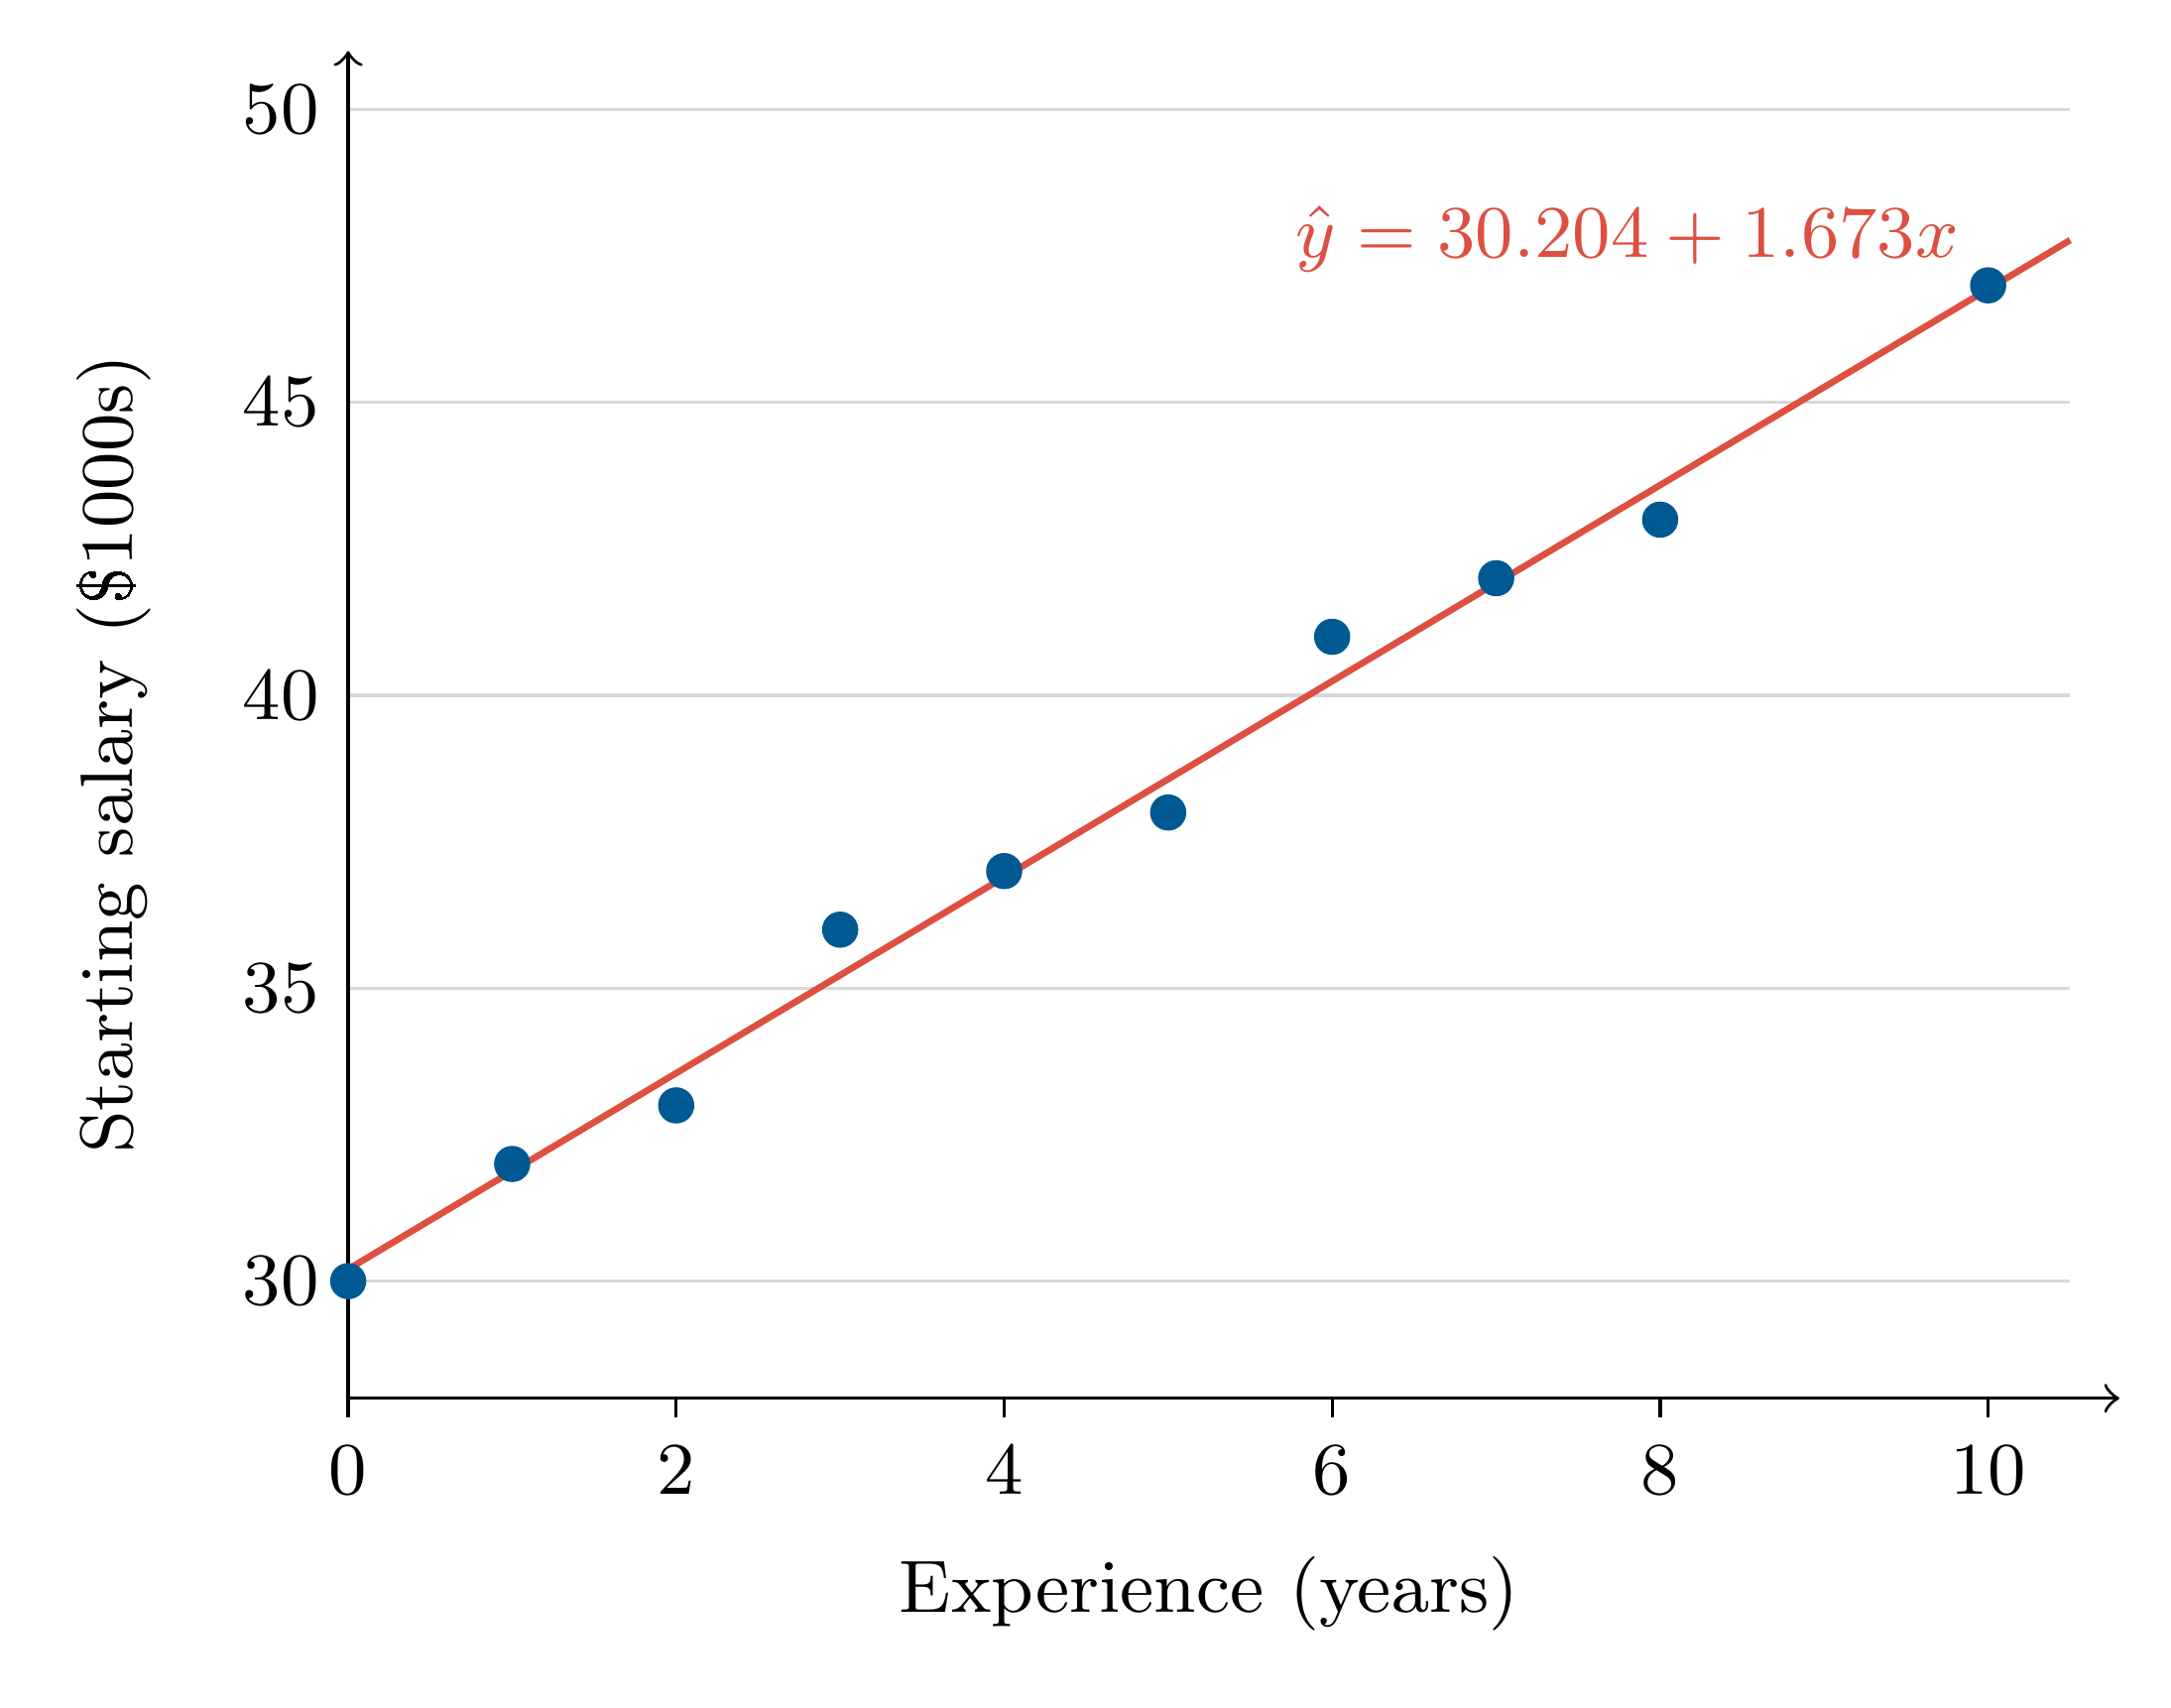
\includegraphics[width=0.56\textwidth]{nm2_scatter_lsrl.png}
    \caption{Experience and starting salary for the 10 sampled teachers, with the least-squares regression line $\hat{y} = 30.204 + 1.673x$.}
    \label{fig:nm2-scatter-lsrl}
\end{figure}

\textbf{Computing in Excel}

You do not need to compute the slope, intercept, and $R^2$ by hand every time.
Excel can produce all of these values at once, along with a scatterplot showing
the line of best fit. Here is how.

First, enter your data into two columns, with experience values in column A and
starting salary values in column B, with headers in row 1. Select both columns,
then insert a scatterplot using \textbf{Insert} $\to$ \textbf{Chart} $\to$
\textbf{Scatter}. Once the chart appears, click on any data point, then select
\textbf{Add Trendline}. In the trendline options panel on the right, choose
\textbf{Linear} and check both \textbf{Display Equation on chart} and
\textbf{Display R-squared value on chart}. Excel will draw the line of best fit
and print the equation and $R^2$ directly on the chart.

\begin{figure}[H]
    \centering
    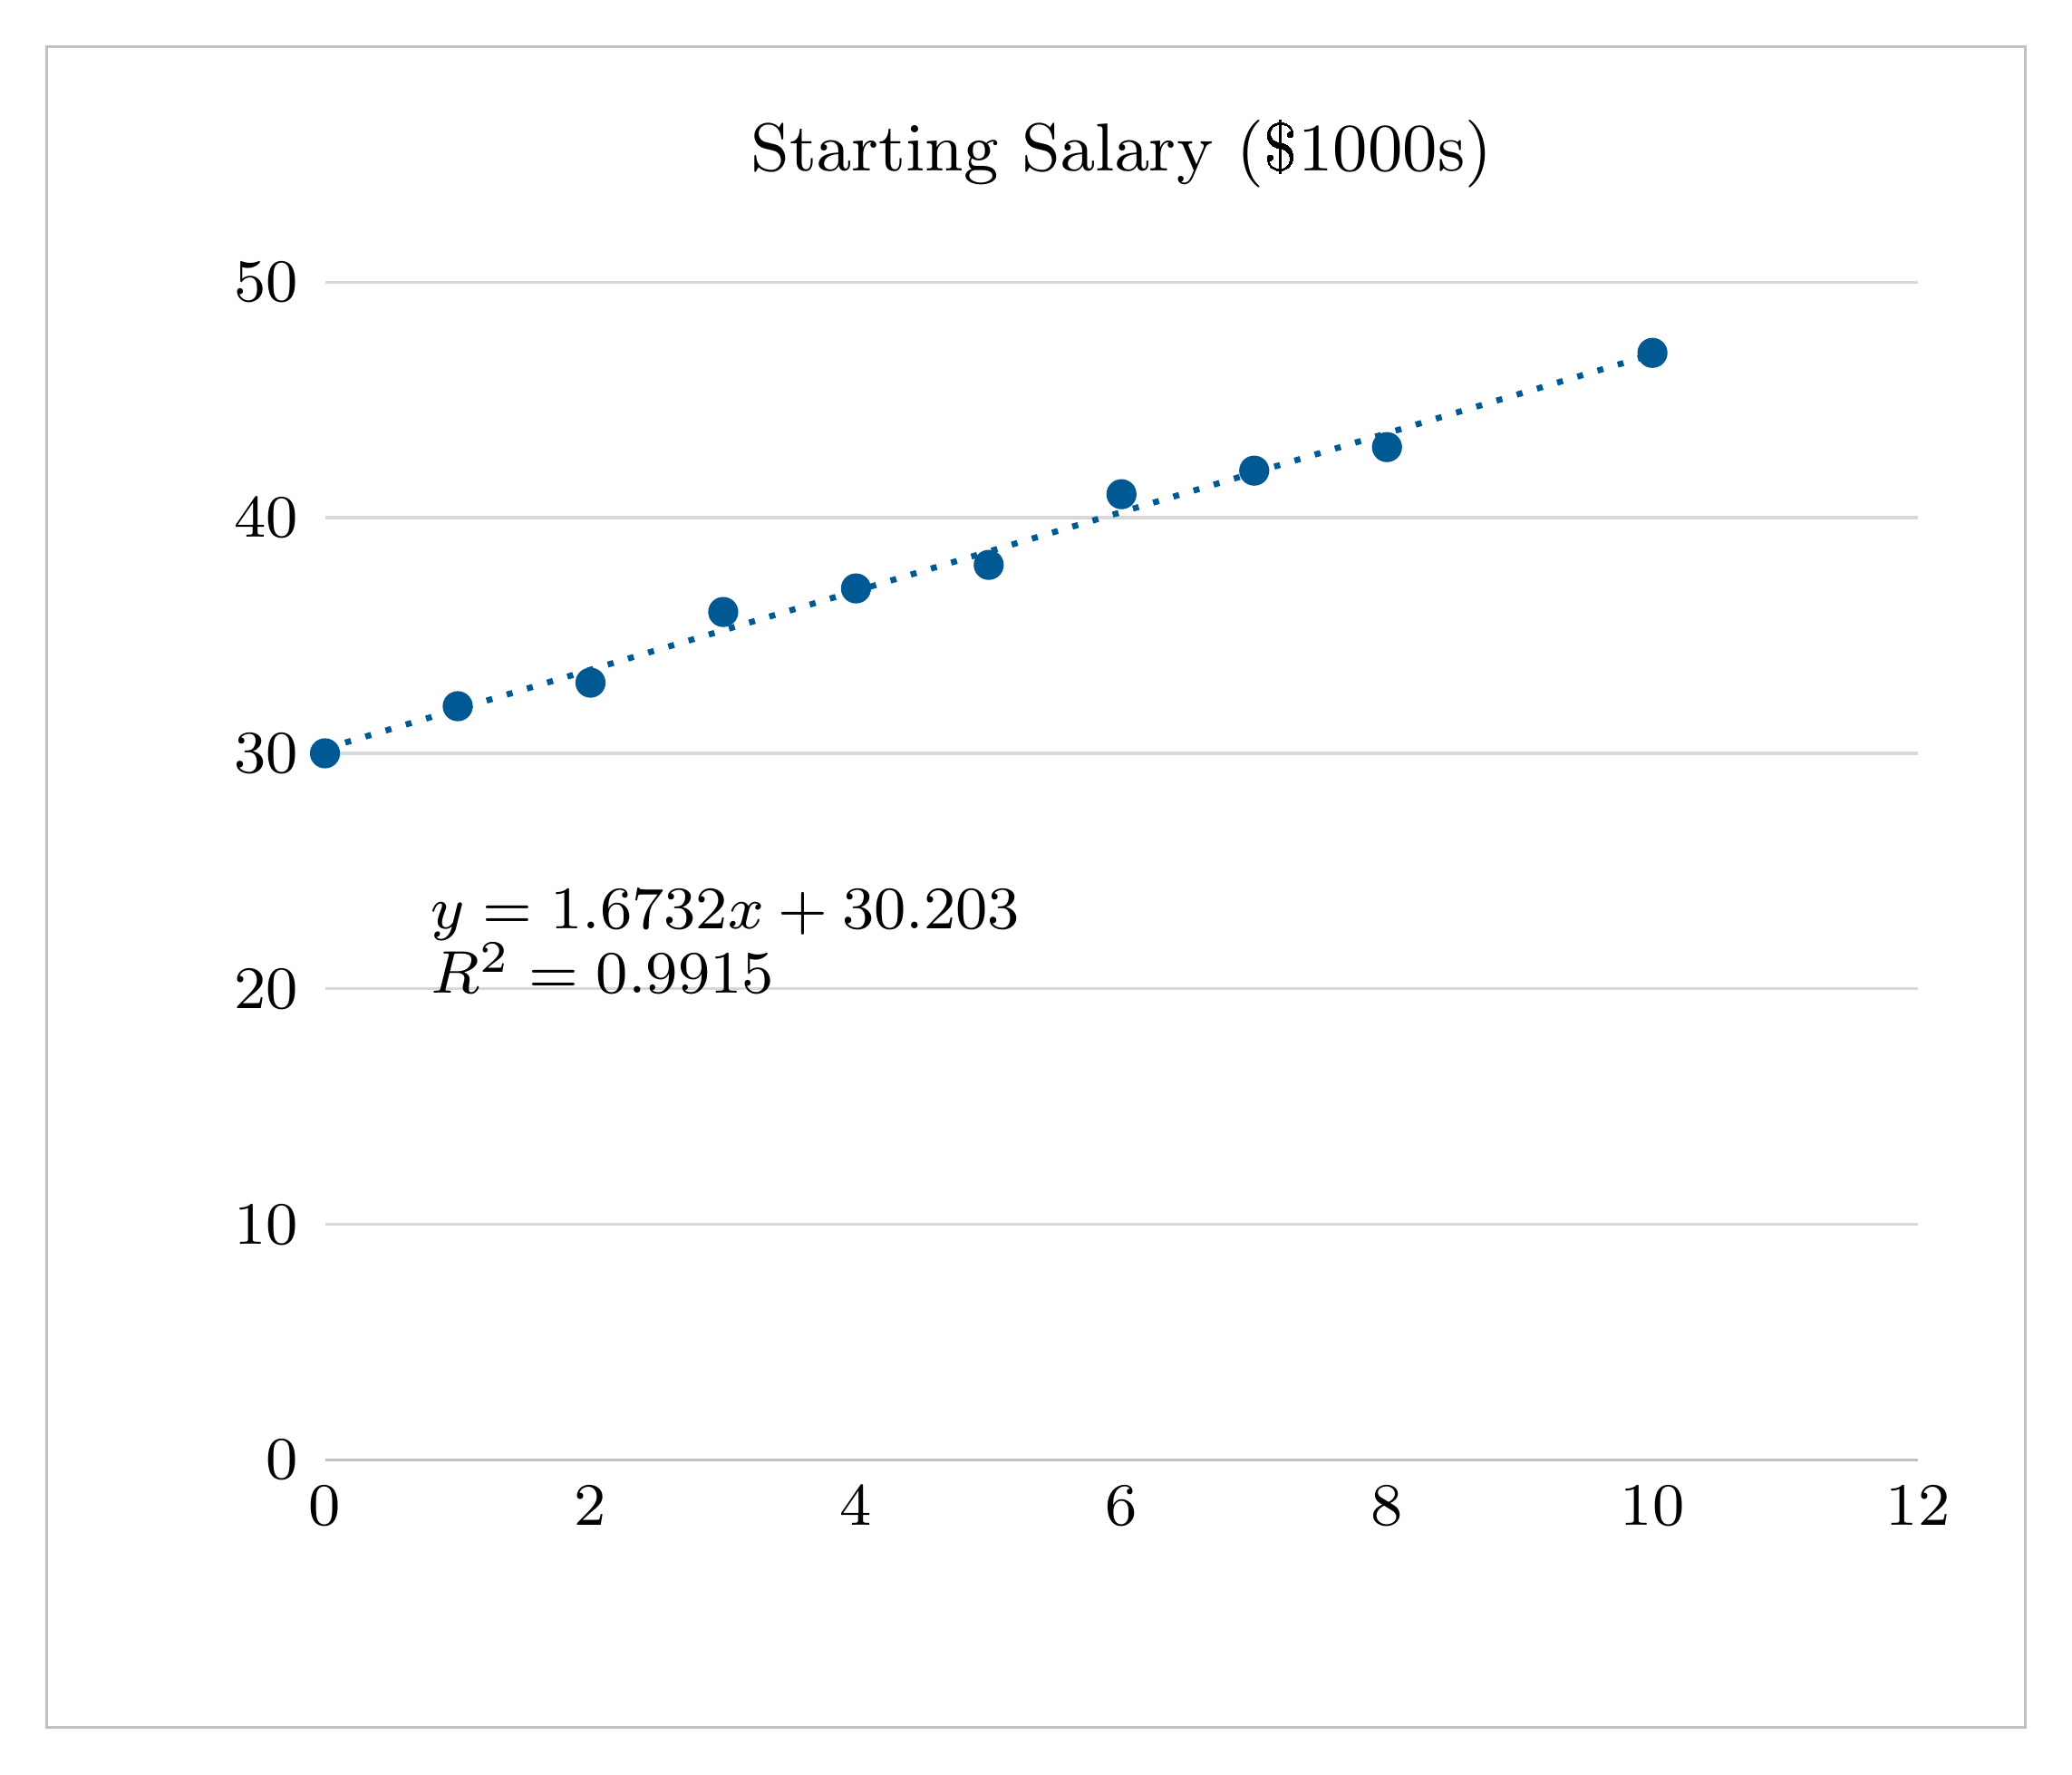
\includegraphics[width=0.58\textwidth]{nm2_excel_trendline.png}
    \caption{Excel scatterplot with a linear trendline, its equation, and $R^2$ displayed on the chart.}
    \label{fig:nm2-excel-trendline}
\end{figure}

To get the full regression output, use the \textbf{Data Analysis} Toolpak. Go to \textbf{Data}
$\to$ \textbf{Data Analysis} $\to$ \textbf{Regression}. Set the Input Y Range
to your salary column and the Input X Range to your experience column. Check
\textbf{Labels} if your columns have headers. Click OK and Excel will produce a
full regression table in a new sheet. The values you need are in the
\textbf{Coefficients} column: the row labelled \textbf{Intercept} gives you $a$,
and the row labelled \textbf{Experience} gives you $b$. The $R^2$ value appears
near the top of the output under \textbf{R Square}.

\begin{figure}[H]
    \centering
    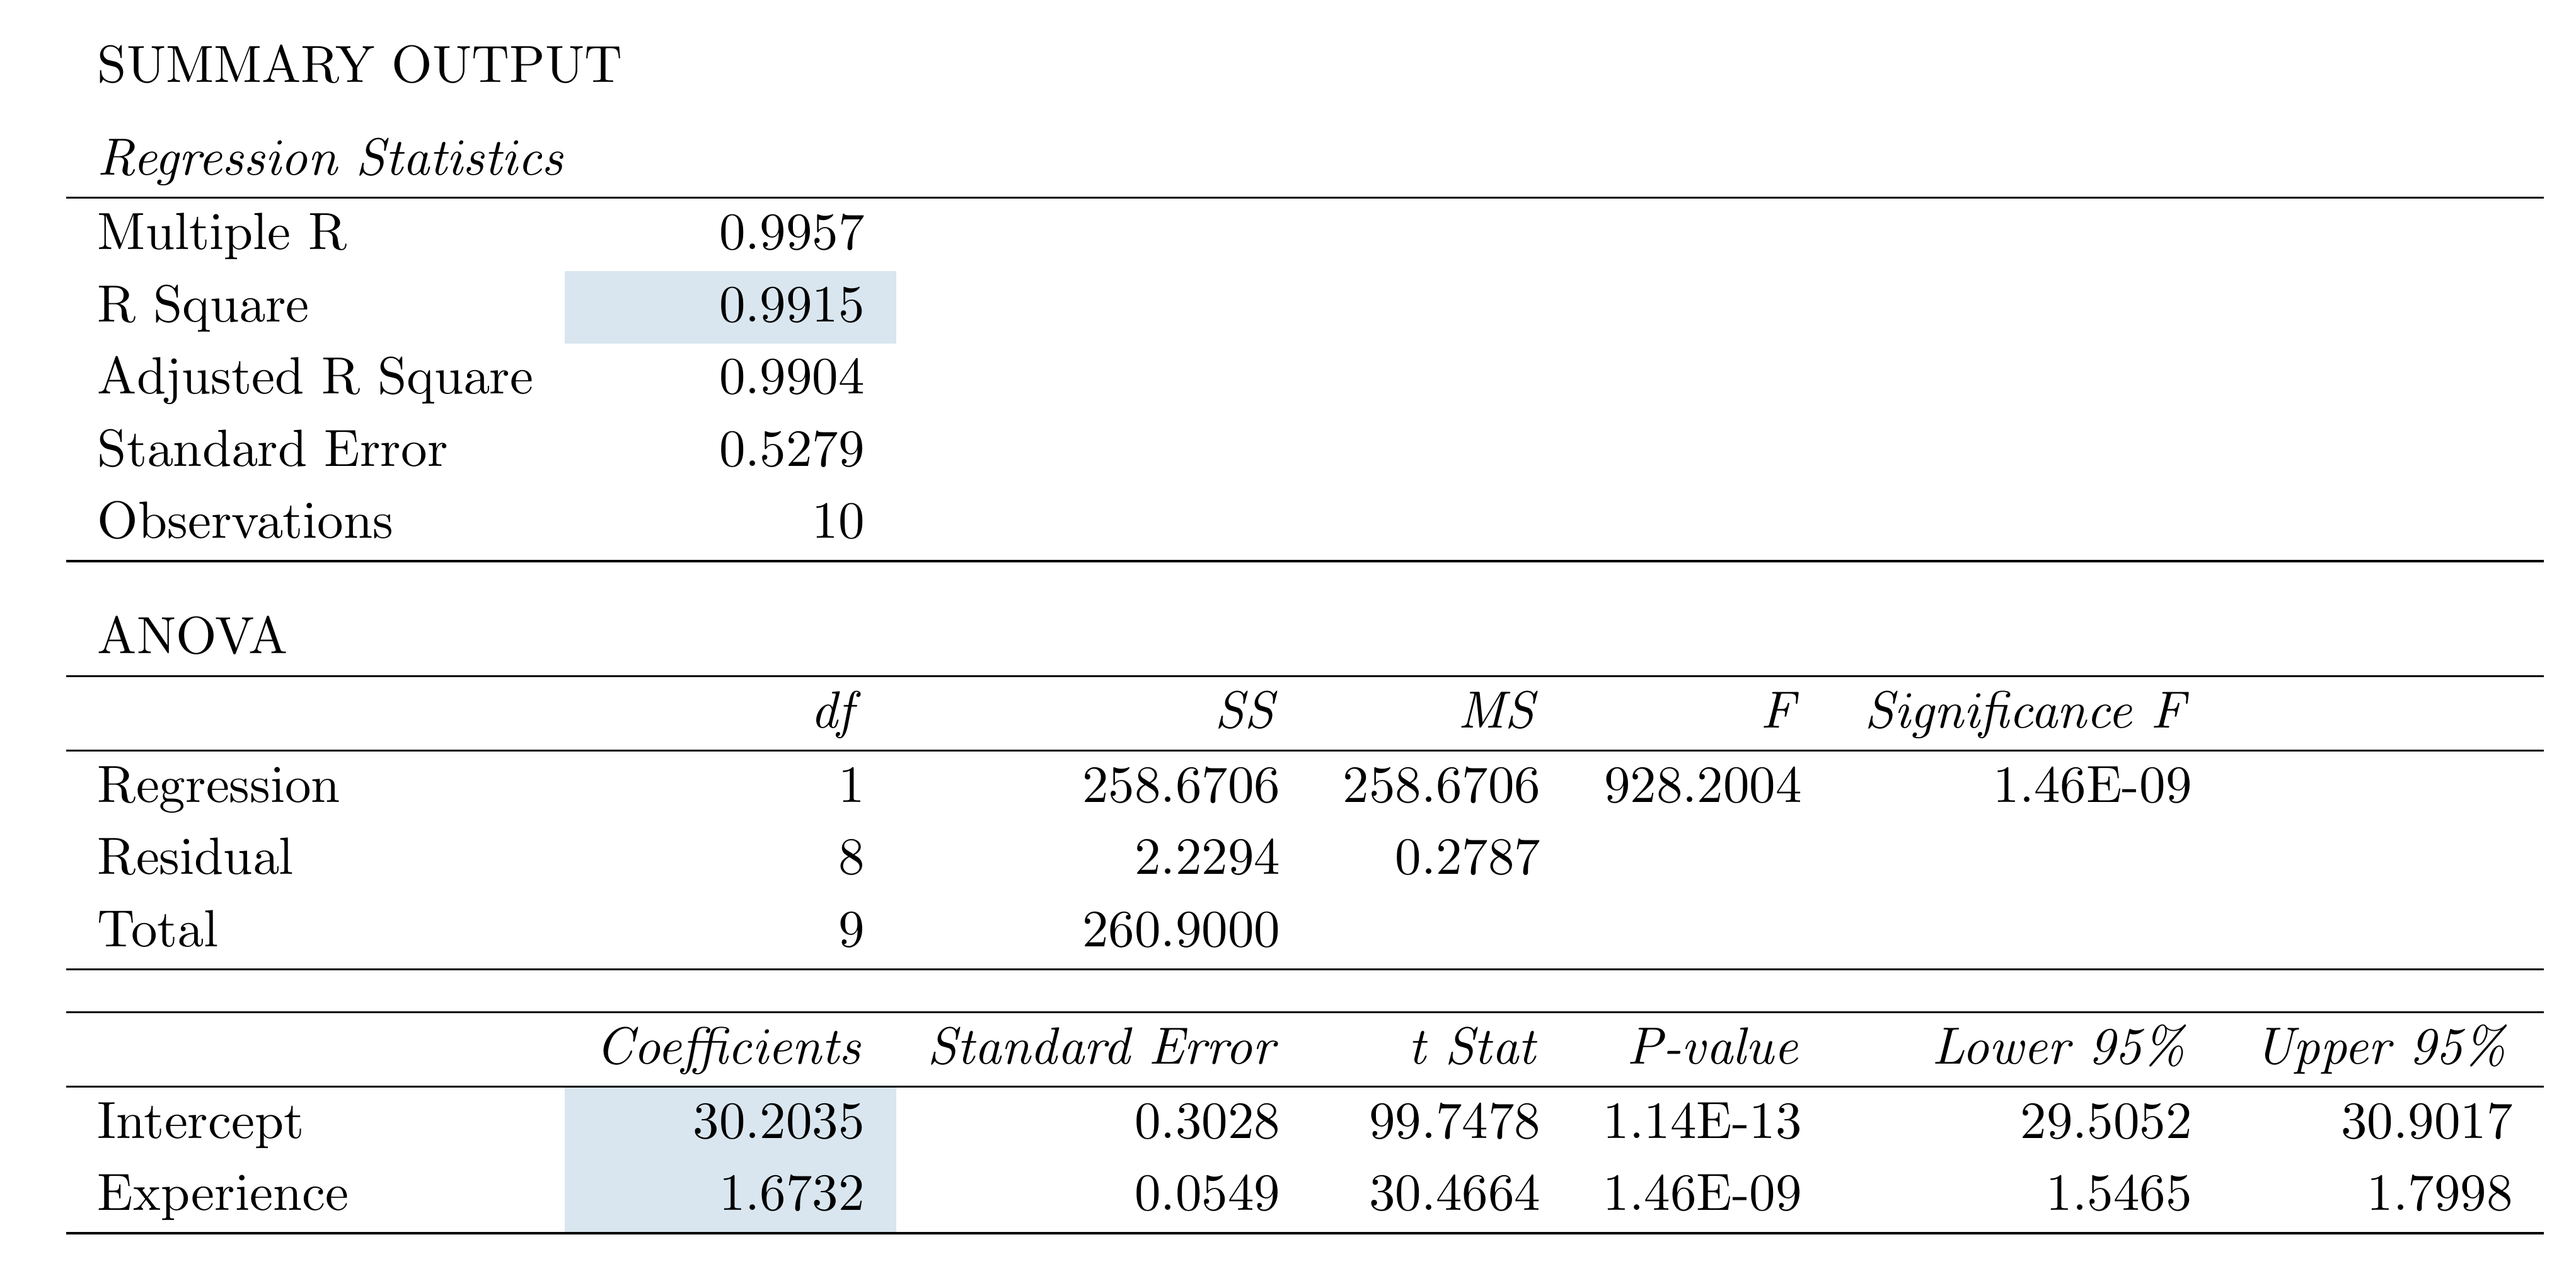
\includegraphics[width=1.0\textwidth]{nm2_regression_output.png}
    \caption{Excel Data Analysis regression output for the teacher data. The highlighted cells give $R^2$, the intercept $a$, and the slope $b$.}
    \label{fig:nm2-regression-output}
\end{figure}

\textbf{Computing in Python}

Python can produce the same regression results as Excel, and a little more
besides. The code below uses \texttt{scipy} for the regression, \texttt{numpy} to
make the points of the line, and \texttt{matplotlib} to draw the scatterplot
with the line of best fit.

\begin{minted}{python}
import numpy as np
from scipy import stats
import matplotlib.pyplot as plt

# Data
experience = [3, 8, 1, 0, 5, 10, 2, 7, 4, 6]
salary     = [36, 43, 32, 30, 38, 47, 33, 42, 37, 41]

# Least-squares regression
slope, intercept, r, p, se = stats.linregress(experience, salary)

print(f"Slope (b):     {slope:.3f}")
print(f"Intercept (a): {intercept:.3f}")
print(f"r:             {r:.4f}")
print(f"R-squared:     {r**2:.4f}")

# Scatterplot with regression line
x_line = np.linspace(0, 10, 100)
y_line = intercept + slope * x_line

plt.scatter(experience, salary, color="steelblue", label="Data")
plt.plot(x_line, y_line, color="firebrick",
         label=f"y = {intercept:.2f} + {slope:.2f}x")
plt.xlabel("Experience (years)")
plt.ylabel("Starting Salary ($1000s)")
plt.title("Experience vs. Starting Salary")
plt.legend()
plt.show()
\end{minted}

Running this code produces the following output:

\begin{verbatim}
Slope (b):     1.673
Intercept (a): 30.203
r:             0.9957
R-squared:     0.9915
\end{verbatim}

\begin{figure}[H]
  \centering
  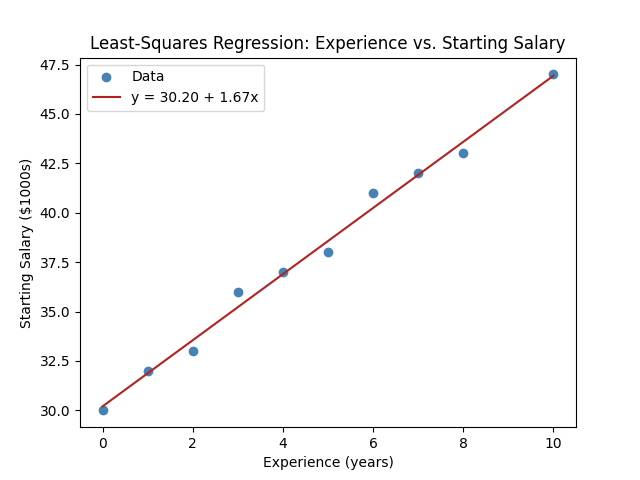
\includegraphics[width=0.8\textwidth]{teacher_sample_figure_1.png}
  \caption{Experience vs. Starting Salary Graph generated from Python}
  \label{fig:teachersamplepython}
\end{figure}

These match the values we computed by hand, up to rounding. The \texttt{stats.linregress}
function does all the heavy lifting! It returns the slope, intercept,
correlation coefficient $r$, a p-value, and the standard error of the slope in
one line. For now, focus on the first four outputs. The p-value and standard
error will become important when we study inference for regression later!
